% WORKAROUND (an update of the geometry package broke beamer...)
\makeatletter\let\ifGm@compatii\relax\makeatother
% end of WORKAROUND


\documentclass[serif]{beamer} %
\usepackage{mathpazo} %
% \usetheme[uttitlepage=false]{ut}
\usetheme[euler=false,titlepage=C]{ut}


\usepackage{arydshln}
\usepackage{tikz-cd}
\usepackage[most]{tcolorbox}

\usepackage[backend=bibtex, style=authoryear, doi=false,isbn=false,url=false]{biblatex}

\usepackage{bm}
\usepackage{color}
\definecolor{theme}{RGB}{0,73,114}

\usepackage{graphicx}
\usepackage{diffcoeff}
\usepackage[most]{tcolorbox}
\usepackage{mathtools}


\setbeamertemplate{caption}{\raggedright\insertcaption\par}


\usepackage[beamer]{hf-tikz}
\usetikzlibrary{calc}

\addtobeamertemplate{footnote}{}{\vspace{2ex}}

\usepackage{xcolor}


% Syntax: \colorboxed[<color model>]{<color specification>}{<math formula>}
\newcommand*{\colorboxed}{}
\def\colorboxed#1#{%
	\colorboxedAux{#1}%
}
\newcommand*{\colorboxedAux}[3]{%
	% #1: optional argument for color model
	% #2: color specification
	% #3: formula
	\begingroup
	\colorlet{cb@saved}{.}%
	\color#1{#2}%
	\boxed{%
		\color{cb@saved}%
		#3%
	}%
	\endgroup
}

% Math macros
\DeclareMathOperator*{\grad}{grad}
\DeclareMathOperator*{\Grad}{Grad}
\DeclareMathOperator*{\Div}{Div}
\renewcommand{\div}{\operatorname{div}}
\DeclareMathOperator*{\Hess}{Hess}
\DeclareMathOperator*{\curl}{curl}
\DeclareMathOperator{\Tr}{Tr}
\DeclareMathOperator{\Dom}{Dom}
\DeclareMathOperator*{\esssup}{ess\,sup}

\newcommand{\bbR}{\mathbb{R}}
\newcommand{\bbF}{\mathbb{F}}
\newcommand{\bbA}{\mathbb{A}}
\newcommand{\bbB}{\mathbb{B}}
\newcommand{\bbS}{\mathbb{S}}

\newcommand*{\norm}[1]{\ensuremath{\left\|#1\right\|}}
\newcommand{\where}{\qquad \text{where} \qquad}
\newcommand{\inner}[3][]{\ensuremath{\left\langle #2, \, #3 \right\rangle_{#1}}}
\newcommand{\bilprod}[2]{\left\langle \left\langle \, #1, #2 \, \right\rangle \right\rangle}
\newcommand{\pder}[2]{\ensuremath{\partial_{#2} #1}}
\newcommand{\dder}[2]{\ensuremath{\delta_{#2} #1}}
\newcommand{\secref}[1]{\S\ref{#1}}
\newcommand{\energy}[1]{\frac{1}{2} \int_{\Omega} \left\{ #1 \right\} \d\Omega}
\newcommand{\crmat}[1]{\ensuremath{\left[#1\right]_\times}}
\newcommand{\fenics}{\textsc{FEniCS}\xspace}
\newcommand{\firedrake}{\textsc{Firedrake}\xspace}

\DeclareMathOperator*{\argmax}{arg\,max}
\DeclareMathOperator*{\argmin}{arg\,min}

\newtheorem{proposition}{Proposition}
\newtheorem{remark}{Remark}
\newtheorem{hypothesis}{Hypothesis}
\newtheorem{assumption}{Assumption}
\newtheorem{conjecture}{Conjecture}


\def\onedot{$\mathsurround0pt\ldotp$}
\def\cddot{% two dots stacked vertically
	\mathbin{\vcenter{\baselineskip.67ex
			\hbox{\onedot}\hbox{\onedot}}%
}}

\renewcommand\bibfont{\scriptsize}


\makeatletter \renewcommand\d[1]{\ensuremath{%
		\;\mathrm{d}#1\@ifnextchar\d{\!}{}}}
\makeatother


\graphicspath{{./images/}}

\bibliography{./biblio_LHMNC}


%% At begin of each section: show current section and all subsections in the section if any
%% At begin of each subsection except first: show only the current section/subsection
\newif\iftocsub
\tocsubtrue
\AtBeginSection[] {
	\begin{frame}[noframenumbering]{Outline}
		\tableofcontents[sectionstyle=show/shaded, subsectionstyle=show/show/hide]
	\end{frame}
	\tocsubfalse
}
\AtBeginSubsection[] {
	\iftocsub
	\begin{frame}[noframenumbering]{Outline}
		\tableofcontents[currentsubsection, sectionstyle=show/shaded, subsectionstyle=show/shaded/hide]
	\end{frame}
	\fi
	\tocsubtrue
}


\title{Mixed finite elements for port-Hamiltonian models of von Kármán beams\\
	\small{7th IFAC Conference on Lagrangian and Hamiltonian method for non linear control}}
%  
\institute[UT]{\inst{1}University of Twente, Enschede (NL) \and \inst{2}ISAE-SUPAERO, Toulouse (FR)}

% \subtitle[Short subtitle]{I am not using any subtitles}
\author[A.~Brugnoli]{\underline{Andrea Brugnoli}\inst{1} \and Ramy Rashad\inst{1} \and Federico Califano\inst{1} \and Stefano Stramigioli\inst{1} \and Denis Matignon\inst{2} } 

\date{\flushright 11-13 October, 2021}
\footlinetext{[A.~Brugnoli]}
% \titlegraphic{\includegraphics[height=1cm]{titlegraphic}}

\utbeamerset{tpboxax=5, tpboxay=20, tpboxawd=100, tpboxbht=30, tpboxbx=5, tpboxby=35, tpboxbwd=120, tpboxbht=30,}

\begin{document}

\maketitle

\begin{frame}{Overview}
	\tableofcontents
\end{frame}

\section{Von-K\'arm\'an theory of thin beams in pH form}

\begin{frame}{Linear vs Von-K\'arm\'an plate theory}

	\begin{columns}
	\begin{column}{.5\textwidth}
			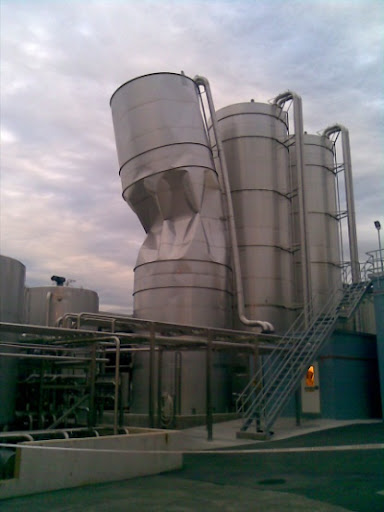
\includegraphics[width=1\columnwidth]{buckling.jpg}
	\end{column}
	\begin{column}{.5\textwidth}

		Geoometrical non-linearities allow describing bifurcations (i.e. buckling).
	\end{column}
	\end{columns}
	
\end{frame}

\begin{frame}{The von-K\'arm\'an assumption}
		
\begin{block}{Basic geometric assumption}
	Out of plane deflection comparable compared to the thickness: $w/h = \mathcal{O}(1)$. \\
\end{block}

\begin{columns}
	\begin{column}{.55\textwidth}
		\includegraphics[width=1\columnwidth]{beam_deflected.eps}
	\end{column}
	\begin{column}{.45\textwidth}
		Aspect ratio: $\delta= h/L$.
		
		The following terms are kept in the expansion:
		\begin{equation*}
		\begin{aligned}
			w/L &= \mathcal{O}(\delta), \\
			u/L &= \mathcal{O}(\delta^2), \\
		\end{aligned}
		\end{equation*}
	\end{column}
\end{columns}

\end{frame}


\begin{frame}{Linear isotropic beams}
	
	The axial and bending behavior are uncoupled if $w/h \ll 1$:
	
	\begin{block}{Axial displacement (wave equation)}
		\begin{equation*}
			\rho A \partial_{tt} u = \partial_x n_{xx}, \qquad n_{xx}=EA \, \partial_x u.
		\end{equation*}
	\end{block}
	
	\begin{block}{Vertical displacement (Euler-Bernoulli equation)}
		\begin{equation*}
			\rho A \partial_{tt} w = -\partial_{xx} m_{xx}, \qquad m_{xx} = EI \partial_{xx} w.
		\end{equation*}
	\end{block}
	For Von-K\'arm\'an beams the two are coupled.
\end{frame}


\begin{frame}{Stresses and Strains in Von-K\'arm\'an beams}
	
Decomposition strain field 
\begin{equation*}
	\varepsilon_{xx} = \overbrace{\tikzmarkin<1>[below right offset={0.05,-0.4},above left offset={-0.05,0.7}]{lm}\diffp{u}{x}\tikzmarkend{lm} +  \tikzmarkin<1>[below right offset={0,-0.4},above left offset={-0.05,0.7}]{nlm}\frac{1}{2} \left(\diffp{w}{x} \right)^2\tikzmarkend{nlm}}^{\varepsilon_{xx}^m} - z \overbrace{\tikzmarkin<1>[below right offset={0.05,-0.4},above left offset={-0.05,0.7}]{lb}\diffp[2]{w}{x}\tikzmarkend{lb}}^{\kappa_{xx}} = \varepsilon_{xx}^m -z \kappa_{xx}.
\end{equation*}

\begin{tikzpicture}[remember picture,overlay]
	% adjust the shift from "col" to move the position of the annotation
	\coordinate (lm-a) at ($(lm)+(-1.5,-1.5)$);
	\coordinate (lm-b) at ($(lm)+(0.4,-1.1)$);
	\node[align=left] (lmstring) at (lm-a) {\small{Linear axial def.}};
	\draw[->, red](lmstring) -| node {} (lm-b);
	
	\coordinate (nlm-a) at ($(nlm)+(-2.2,-2)$);
	\coordinate (nlm-b) at ($(nlm)+(0.8,-1.1)$);
	\node[align=left] (nlmstring) at (nlm-a) {\small{Non-linear axial def.}};
	\draw[->, red](nlmstring) -| node {} (nlm-b);
	
	\coordinate (lb-a) at ($(lb)+(+2,-2)$);
	\coordinate (lb-b) at ($(lb)+(0.3,-1.1)$);
	\node[align=right] (lbstring) at (lb-a) {\small{Linear bending def.}};
	\draw[->, red](lbstring) -| node {} (lb-b);
\end{tikzpicture}
\vspace{1cm}\\

\begin{block}{Membrane and bending stresses (isotropic material)}
	\begin{equation*}
		\begin{aligned}
			n_{xx} &= \int_S E \d{S} \varepsilon_{xx}^m = EA \varepsilon_{xx}^m, \quad\quad\;\;\; \text{Axial stress resultant}\\
			 m_{xx} &= -\int_S E z^2 \d{S}\kappa_{xx} = EI \kappa_{xx},  \quad \text{Bending stress resultant}
		\end{aligned}
	\end{equation*}
\end{block}

\end{frame}


\begin{frame}{Port-Hamiltonian Von-K\'arm\'an beams}
	
\begin{block}{Dynamics}
	\begin{equation*}
		\begin{aligned}
			\rho A \partial_{tt}{u} &= \partial_x \tikzmarkin<1>[below right offset={-0.05,-0.15},above left offset={-0.0,0.3}]{cp1}n_{xx}\tikzmarkend{cp1}, \\
			\rho A \partial_{tt}{w} &= -\partial^2_{xx} m_{xx} + \partial_x(\tikzmarkin<1>[below right offset={-0.05,-0.15},above left offset={-0.0,0.3}]{cp2}n_{xx}\tikzmarkend{cp2} \partial_x w),
		\end{aligned} 
	\end{equation*}
\end{block}

\begin{block}{Energy and coenergy variables}
	Same selection as usual:
	\begin{equation*}
		\begin{aligned}
			\alpha_u &= \rho A \partial_t{u}, \\
			\alpha_w &= \rho A \partial_t{w},\\
		\end{aligned} \qquad
		\begin{aligned}
			\alpha_\varepsilon &= \varepsilon_{xx}^m, \\
			\alpha_\kappa &= \kappa_{xx}.
		\end{aligned}
	\end{equation*}
	Linear constitutive relation $\bm{e} = \mathcal{Q} \bm{\alpha}$ with
	\begin{equation*}
		\mathcal{Q} = \mathrm{Diag}\left[\rho A, \; C_a, \; \rho A, \; C_b\right]^{-1}, \quad C_a = (EA)^{-1}, \quad C_b = (EI)^{-1},
	\end{equation*}
where $C_a, C_b$ are the axial and bending compliances.
\end{block}

\end{frame}

\begin{frame}{The port-Hamiltonian realization}
	To close the system, variable $w$ has to be accessible. 
	\begin{equation*}
		\frac{\partial}{\partial t}
		\begin{pmatrix}
			\alpha_u \\
			\alpha_\varepsilon \\
			\alpha_w \\
			\alpha_\kappa \\
			w \\
		\end{pmatrix} = 
		\underbrace{\begin{bmatrix}
				0 & \partial_x & 0 & 0 & 0\\
				\partial_x & 0 & \colorboxed{blue}{(\partial_x w) \, \partial_x}  & 0 & 0 \\
				0 & \colorboxed{blue}{\partial_x(\cdot \, \partial_x w)} & 0 & -\partial_{xx}^2 & -1 \\
				0 & 0 & \partial_{xx}^2 & 0 & 0 \\ 
				0 & 0 & 1 &  & 0 \\
		\end{bmatrix}}_{\mathcal{J}}
		\begin{pmatrix}
			e_u \\
			e_\varepsilon \\
			e_w \\
			e_\kappa \\
			\delta_w H  \\
		\end{pmatrix}.
	\end{equation*}

\begin{proposition}
	The operator $\mathcal{J}$ is formally skew-adjoint.
\end{proposition}
	The construction is analogous for plate problems\vspace{.1cm}\footfullcite{brugnoli2022enoc}.
\end{frame}

\begin{frame}{Energy rate and boundary conditions}
	
	\begin{proposition}{The energy rate reads}
		\begin{equation*}
			\dot{H} = \inner[\partial\Omega]{e_u}{e_\varepsilon} + \inner[\partial\Omega]{e_w}{e_\varepsilon \partial_x w -\partial_x e_\kappa} + \inner[\partial\Omega]{\partial_x e_w}{e_\kappa}.
		\end{equation*}
	with $\Omega = [0, \; L]$ and $\inner[\Omega]{\cdot}{\cdot}$ the $L^2$ inner product.
	\end{proposition}

\begin{table}[h]
	Boundary conditions classification
	\centering
	\begin{tabular}{c|c|c|c}
		\hline 
		BCs & Traction & \multicolumn{2}{c}{Bending} \\ 
		\hline 
		Dirichlet BCs. & $e_u\vert_0^L$ & $e_w\vert_0^L$  & $\partial_x e_w\vert_0^L$  \\
		Neumann BCs. & $e_\varepsilon\vert_0^L$ & $e_\varepsilon \partial_x w -\partial_x e_\kappa\vert_0^L$ & $e_\kappa\vert_0^L$ \\ 
		\hline 
	\end{tabular} 
\end{table}

Same bcs. as in \cite{puel1996} for global existence and uniqueness result.
\end{frame}


\section{Numerical discretization}

\begin{frame}{Pure coenergy formulation}
	
	\begin{block}{Coenergy formulation for linear constitutive equations}
		If the $\mathcal{Q}$ operator is inverted:
		\begin{equation*}
			\begin{pmatrix}
				\rho A \dot{e}_u \\
				C_a \dot{e}_\varepsilon \\
				\rho A \dot{e}_w \\
				C_b \dot{e}_\kappa \\
				\dot{w} \\
			\end{pmatrix} = 
			\begin{bmatrix}
				0 & \partial_x & 0 & 0 & 0\\
				\partial_x & 0 & \partial_x w \, \partial_x & 0 & 0 \\
				0 & \partial_x(\cdot \, \partial_x w) & 0 & -\partial_{xx}^2 & -1 \\
				0 & 0 & \partial_{xx}^2 & 0 & 0 \\ 
				0 & 0 & 1 & 0 & 0 \\
			\end{bmatrix}
			\begin{pmatrix}
				e_u \\
				e_\varepsilon \\
				e_w \\
				e_\kappa \\
				\delta_w H \\
			\end{pmatrix}.
		\end{equation*}
	\end{block}
In the sequel, the quantity $\delta_w H$ is removed as no displacement dependent potential (e.g. gravity) is considered
	
\end{frame}

\begin{frame}{Weak formulation}
	
	Introducing test functions and integrating by parts the first, third and fourth, we get the weak formulation.
	
	\begin{block}{Weak formulation}
		\only<1>{Find $(e_u, e_w, e_\kappa, w) \in H^1(\Omega), \, e_\varepsilon \in L^2(\Omega)$ such that 
			\begin{equation*}
				\begin{aligned}
					\inner[\Omega]{\psi_u}{\rho A \, \dot{e}_u} &= -\inner[\Omega]{\partial_x \psi_u}{ e_\varepsilon} +  \inner[\partial\Omega]{\psi_u}{e_\varepsilon}. \\
					\inner[\Omega]{\psi_\varepsilon}{C_a \, \dot{e}_\varepsilon} &= \inner[\Omega]{\psi_\varepsilon}{\partial_x e_u} + \inner[\Omega]{\psi_\varepsilon}{\partial_x w \, \partial_x e_w}, \\
					\inner[\Omega]{\psi_w}{\rho A\dot{e}_w} &= -\inner[\Omega]{\partial_x \psi_w \partial_x w}{e_\varepsilon} + \inner[\Omega]{\partial_{x} \psi_w}{\partial_{x} e_\kappa} \\
					&\quad +\inner[\partial\Omega]{\psi_w}{e_\varepsilon \partial_x w - \partial_x e_\kappa}, \\
					\inner[\Omega]{\psi_\kappa}{C_b \, \dot{e}_\kappa} &= - \inner[\Omega]{\partial_{x} \psi_\kappa}{\partial_{x} e_w} + \inner[\partial\Omega]{\psi_\kappa}{\partial_x e_w}, \\
					\inner[\Omega]{\psi}{\dot{w}} &= \inner[\Omega]{\psi}{e_w}. \\
				\end{aligned}
			\end{equation*}
			holds $\forall (\psi_u, \psi_w, \psi_\kappa, \psi) \in H^1(\Omega), \, \forall \psi_\varepsilon \in L^2(\Omega)$.}
		\only<2>{
		Find $\bm{e} =(e_u,  e_\varepsilon, e_w, e_\kappa) \in H^1\times L^2\times H^1\times H^1$ such that 
		\begin{equation*}
			\begin{aligned}
				m(\bm{\psi}, \partial_t \bm{e}) &= j_w(\bm{\psi}, \bm{e}) + b(\bm{\psi})\mathbf{u},\\
				\partial_t w &= \begin{bmatrix}
					0 & 0 & 1 & 0
				\end{bmatrix}\bm{e}, \\
				\mathbf{y} &= b^\top(\bm{e}),
			\end{aligned} 
		\end{equation*}
		$\forall \bm{\psi} \in H^1\times L^2\times H^1\times H^1:= X$
		\begin{itemize}
			\item $m$ is a symmetric, coercive, bilinear form;
			\item $j_w$ is a skew-symmetric bilinear form modulated by $w$;
			\item $b: X \rightarrow \bbR^6$ vector-valued functional.
		\end{itemize}  
	}
	\end{block}
\end{frame}

\begin{frame}{Mixed finite element construction\footcite{arnold2006acta}}
	\textcolor{blue}{Crucial concept: Hilbert complex $H^1 \xrightarrow{\partial_x} L^2$.} \\
	\begin{block}{Key requirements for mixed Galerkin approximation}
		
	\begin{itemize}
		\item The subspaces $H^1_h \subset H^1, \; L^2_h \subset L^2$ form a subcomplex $H^1_h \xrightarrow{\partial_x} L^2_h$ \hspace{1cm}(i.e. $\partial_x H^1_h \subset L^2_h$).
		\item they admit bounded linear projections $\pi_h^{H^1}: H^1 \rightarrow  
		H^1_h$  and $\pi_h^{L^2}: L^2 \rightarrow  
		L^2_h$ which commute with $\partial_x$:
		\vspace*{-\baselineskip}\vspace*{3pt}
		\[\partial_x \pi_h^{H^1} = \pi_h^{L^2} \partial_x.\]
	\end{itemize}
	\end{block}

	Satisfied for $CG_k \xrightarrow{\partial_x} DG_{k-1}$ 
	\begin{equation*}
		\begin{aligned}
			\mathrm{CG}_k &= \{u \in H^1(\Omega) | \: \forall \text{edge in the mesh}, \; u|_{\text{edge}} \in P_k\}, \\
			\mathrm{DG}_{k-1} &= \{u \in L^2(\Omega) | \: \forall \text{edge in the mesh}, \; u|_{\text{edge}} \in P_{k-1}\}, \\
		\end{aligned}
	\end{equation*}
	where $P_k$ space of polynomials of degree $k$.
	\vspace{.1cm}
\end{frame}

\begin{frame}{Finite element choice and final system}
	For the proposed weak formulation, the FE spaces become
	\begin{equation*}
			e_u^h \in \mathrm{CG}_{2k-1}, \qquad
			e_{\varepsilon}^h \in \mathrm{DG}_{2k-2}, \qquad 
			(e_w^h, \; e_\kappa^h, \; w^h) \in CG_{k}, \quad k\ge 1.
	\end{equation*}
Implications:
\begin{itemize}
	\item Subcomplex property for the linear part: $\partial_x \mathrm{CG}_{k-1} \subset \mathrm{DG}_{2k-2}$.
	\item The non linear part respects
	$$\partial_x \mathrm{CG}_k \cdot  \partial_x \mathrm{CG}_k \subset \mathrm{DG}_{2k-2}.$$
\end{itemize}

\begin{block}{Finite dimensional system (Galerkin projection)}
		\begin{equation*}
		\begin{aligned}
			\mathbf{M} \dot{\mathbf{e}} &= \mathbf{J}(\mathbf{w})\mathbf{e} + \mathbf{B}\mathbf{u}, \\
			\dot{\mathbf{w}} &= \begin{bmatrix}
				\mathbf{0} & \mathbf{0} & \mathbf{I} & \mathbf{0} \\
			\end{bmatrix} \mathbf{e}, \\
			\mathbf{y} &= \mathbf{B}^\top \mathbf{e}.
		\end{aligned}
	\end{equation*}
\end{block}

\end{frame}


\section{Numerical convergence study}

\begin{frame}{Manufactured solution}
	The following manufactured solution is considered
	\begin{equation*}
		\begin{aligned}
			u^{\text{ex}} &= x^3[1-(x/L)^3] \sin(2 \pi t), \qquad
			w^{\text{ex}} &= \sin(\pi x/L)\sin(2 \pi t), 
		\end{aligned}
	\end{equation*}
	together with the boundary conditions
	\begin{equation*}
		u\vert_0^L = 0, \quad w\vert_0^L =0, \quad m_{xx}\vert_{0}^L=0.
	\end{equation*}
A Crank-Nicholson scheme is used for time integration.
\begin{block}{Convergence measure}
	The discrete time-space norm $L^\infty_{\Delta t} (\mathcal{X}) (\mathcal{X} = H^1 \text{or } L^2)$ is used to measure convergence
	\[
	||\cdot ||_{L^\infty (\mathcal{X})} \approx || \cdot ||_{L^\infty_{\Delta t} (\mathcal{X})} = \max_{t \in t_i} ||\cdot||_{\mathcal{X}},
	\]
	where $t_i$ are the discrete simulation instants.
\end{block}

\end{frame}

\begin{frame}{Results}
	\only<1>{
		\begin{figure}[b]
			\begin{minipage}[b]{0.58\linewidth}
				\centering
				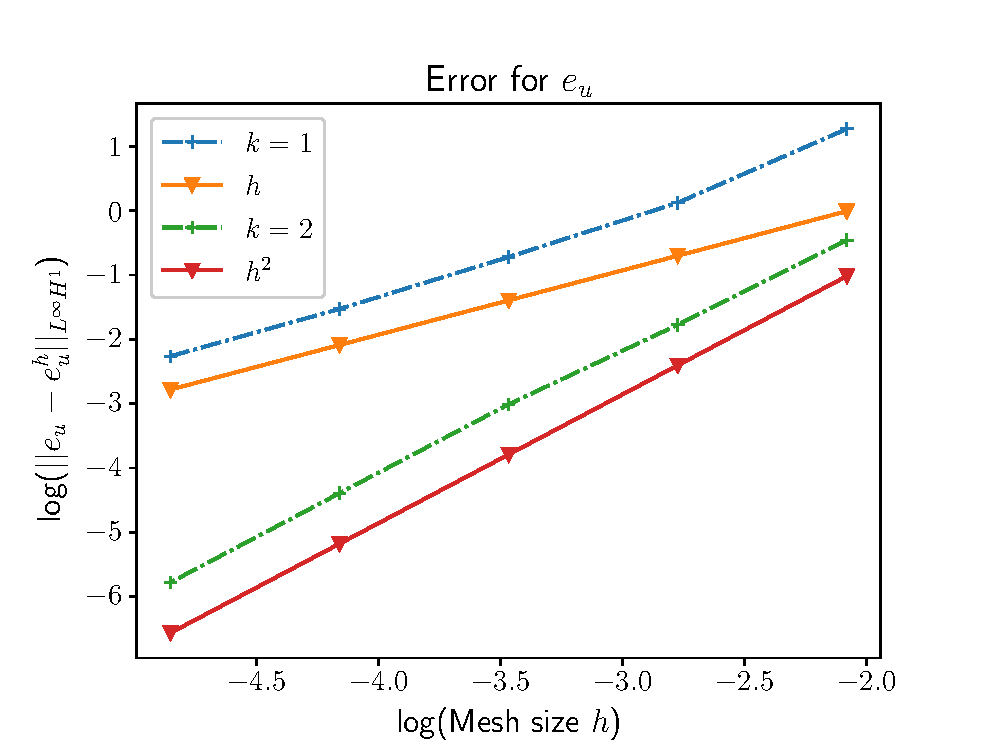
\includegraphics[width=1\textwidth]{u_dot.eps}
				\caption{$L^\infty_{\Delta t} (H^1)$ error for $e_u$.}
			\end{minipage}
			\begin{minipage}[b]{0.4\linewidth}
				\centering
				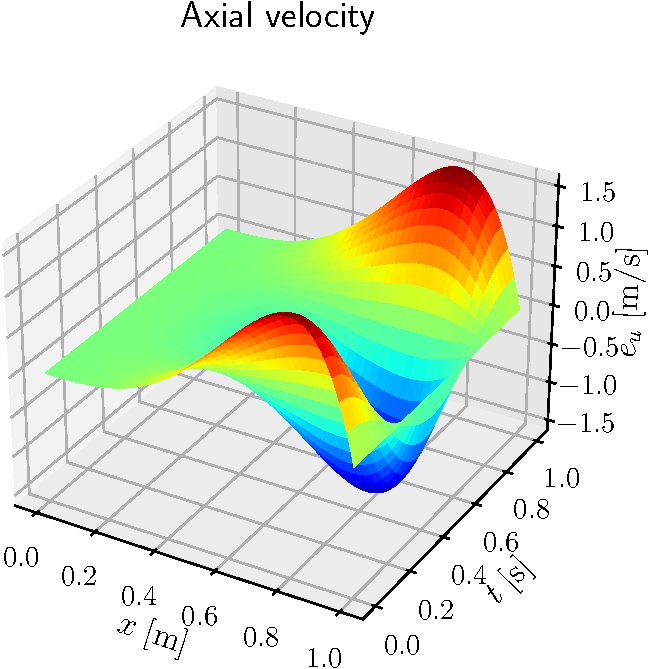
\includegraphics[width=1\textwidth]{plot_e_u_cropped.pdf}
				\caption{$e_u^h$ ($h=2^{-5}, k=2$).}
			\end{minipage}
		\end{figure}
	}
	\only<2>{
		\begin{figure}[b]
			\begin{minipage}[b]{0.58\linewidth}
				\centering
				\includegraphics[width=1\textwidth]{n_xx.eps}
				\caption{$L^\infty_{\Delta t} (L^2)$ error for $e_\varepsilon$.}
			\end{minipage}
			\begin{minipage}[b]{0.4\linewidth}
				\centering
				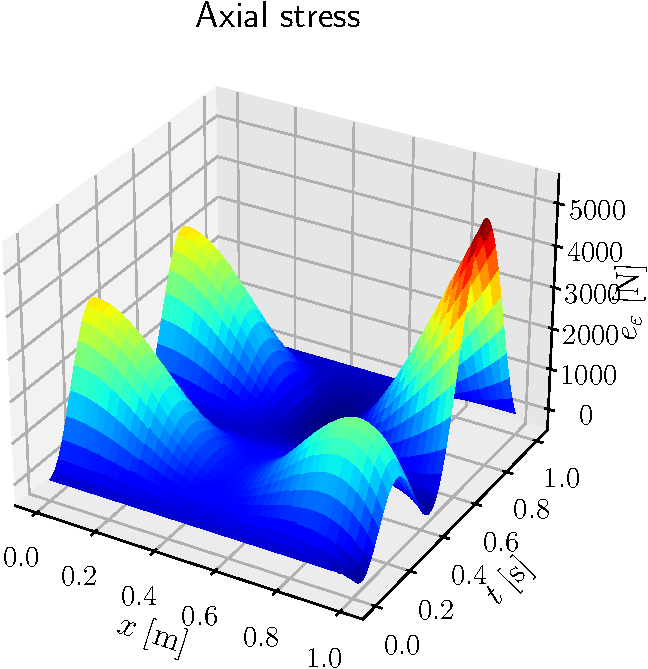
\includegraphics[width=1\textwidth]{plot_e_eps_cropped.pdf}
				\caption{$e_\varepsilon^h$ for $h=2^{-5}, k=2$.}
			\end{minipage}
		\end{figure}
	}
	\only<3>{
		\begin{figure}[b]
			\begin{minipage}[b]{0.58\linewidth}
				\centering
				\includegraphics[width=1\textwidth]{w_dot.eps}
				\caption{$L^\infty_{\Delta t} (H^1)$ error for $e_w$.}
			\end{minipage}
			\begin{minipage}[b]{0.4\linewidth}
				\centering
				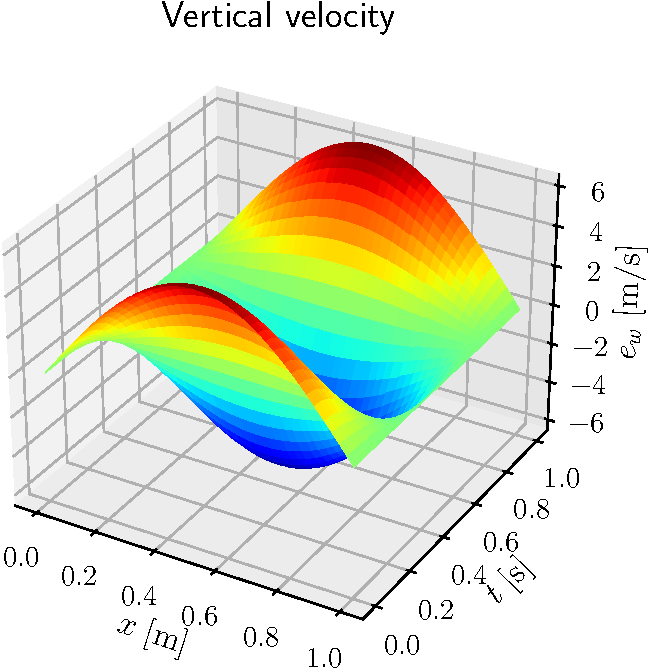
\includegraphics[width=1\textwidth]{plot_e_w_cropped.pdf}
				\caption{$e_w^h$ for $h=2^{-5}, k=2$.}
			\end{minipage}
		\end{figure}
	}
	\only<4>{
		\begin{figure}[b]
			\begin{minipage}[b]{0.58\linewidth}
				\centering
				\includegraphics[width=1\textwidth]{m_xx.eps}
				\caption{$L^\infty_{\Delta t} (H^1)$ error for $e_\kappa$.}
			\end{minipage}
			\begin{minipage}[b]{0.4\linewidth}
				\centering
				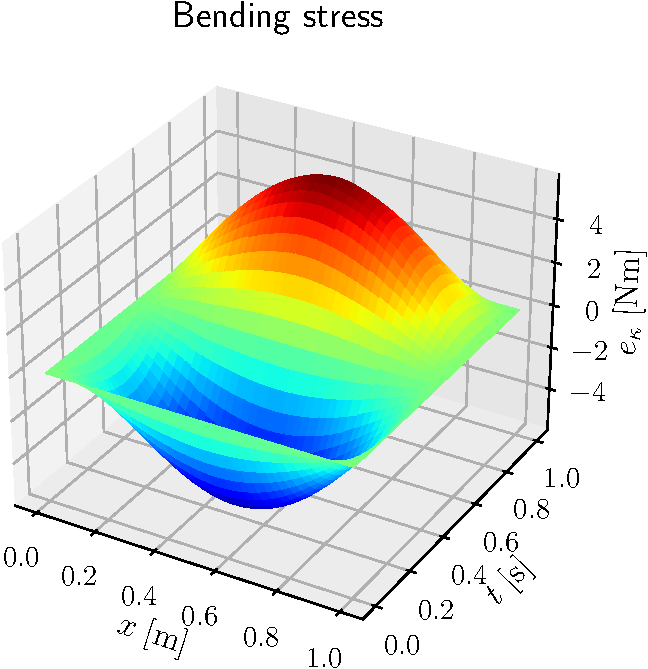
\includegraphics[width=1\textwidth]{plot_e_kap_cropped.pdf}
				\caption{$e_\kappa^h$ for $h=2^{-5}, k=2$.}
			\end{minipage}
		\end{figure}
	}
\end{frame}

\begin{frame}{Conclusion and Outlook}
\begin{itemize}
	\item First step into pH non linear mechanics. The geometrical non linearities belong to the interconnection operator.
	\item Natural extension for the 2D case (fancier FE).
	\item Can be used to study more complex phenomena. The discretization method guarantees energy conservation.
\end{itemize}
\end{frame}

\begin{frame}[allowframebreaks]{References}\label{lastslide}
	\printbibliography
\end{frame}


\begin{frame}{Port-Hamiltonian von-K\'arm\'an plates}
	\begin{equation*}
		%\diffp{}{t}
		\frac{\partial}{\partial t}
		\begin{pmatrix}
			\bm{\alpha}_u \\
			\bm{A}_\varepsilon \\
			w \\
			\alpha_w \\
			\bm{A}_\kappa
		\end{pmatrix} = 
		\underbrace{\begin{bmatrix}
				\bm{0} & \Div & \bm{0} & \bm{0} & \bm{0}\\
				\Grad & \bm{0} & \bm{0} & -\mathcal{C}(w)^* & \bm{0} \\
				0 & 0 & 0 & 1 & 0 \\
				0 & \mathcal{C}(w) & -1 & 0 & -\div\Div \\
				\bm{0} & \bm{0} & \bm{0} & \Grad\grad & \bm{0} \\ 
		\end{bmatrix}}_{\mathcal{J}}
		\begin{pmatrix}
			\delta_{\bm\alpha_u} H \\
			\delta_{\bm{A}_\varepsilon} H \\
			\delta_{w} H \\
			\delta_{\alpha_w} H \\
			\delta_{\bm{A}_\kappa} H
		\end{pmatrix},
	\end{equation*}
where 
\begin{equation*}
	\begin{aligned}
		\mathcal{C}(w)(\bm{T}) &= \div(\bm{T} \grad w), \\
		\mathcal{C}(w)^*(\cdot) &= -\frac{1}{2} \left[\grad (\cdot) \otimes \grad(w) + \grad(w) \otimes \grad(\cdot) \right].
	\end{aligned}
\end{equation*}

\end{frame}




\end{document}

